\documentclass[a4paper,12pt]{article}
\usepackage{caption}
\usepackage{float}
\usepackage{graphicx}
%%%%%%%%%%%%%%%%%%%%%%%%%%%%%%%%%%%%%%%%%
% Contract
% Structural Definitions File
% Version 1.0 (December 8 2014)
%
% Created by:
% Vel (vel@latextemplates.com)
% 
% This file has been downloaded from:
% http://www.LaTeXTemplates.com
%
% License:
% CC BY-NC-SA 3.0 (http://creativecommons.org/licenses/by-nc-sa/3.0/)
%
%%%%%%%%%%%%%%%%%%%%%%%%%%%%%%%%%%%%%%%%%

%----------------------------------------------------------------------------------------
%	PARAGRAPH SPACING SPECIFICATIONS
%----------------------------------------------------------------------------------------

\setlength{\parindent}{0mm} % Don't indent paragraphs

\setlength{\parskip}{2.5mm} % Whitespace between paragraphs

%----------------------------------------------------------------------------------------
%	PAGE LAYOUT SPECIFICATIONS
%----------------------------------------------------------------------------------------

\usepackage{geometry} % Required to modify the page layout

\setlength{\textwidth}{16cm} % Width of the text on the page
\setlength{\textheight}{24.5cm} % Height of the text on the page

\setlength{\oddsidemargin}{0cm} % Width of the margin - negative to move text left, positive to move it right

% Uncomment for offset margins if the 'twoside' document class option is used
%\setlength{\evensidemargin}{-0.75cm} 
%\setlength{\oddsidemargin}{0.75cm}

\setlength{\topmargin}{-1.25cm} % Reduce the top margin

%----------------------------------------------------------------------------------------
%	FONT SPECIFICATIONS
%----------------------------------------------------------------------------------------

% If you are running Apple OS X, uncomment the next 4 lines and comment/delete the block below, you will now need to compile with XeLaTeX but your document will look much better

%\usepackage[cm-default]{fontspec}
%\usepackage{xunicode}

%\setsansfont[Mapping=tex-text,Scale=1.1]{Gill Sans}
%\setmainfont[Mapping=tex-text,Scale=1.0]{Hoefler Text}

%-------------------------------------------

\usepackage[utf8]{inputenc} % Required for including letters with accents
\usepackage[T1]{fontenc} % Use 8-bit encoding that has 256 glyphs

\usepackage{avant} % Use the Avantgarde font for headings
\usepackage{mathptmx} % Use the Adobe Times Roman as the default text font together with math symbols from the Sym­bol, Chancery and Com­puter Modern fonts

%----------------------------------------------------------------------------------------
%	SECTION TITLE SPECIFICATIONS
%----------------------------------------------------------------------------------------

\usepackage{titlesec} % Required for modifying section titles

\titleformat{\section} % Customize the \section{} section title
{\sffamily\large\bfseries} % Title font customizations
{\thesection} % Section number
{16pt} % Whitespace between the number and title
{\large} % Title font size
\titlespacing*{\section}{0mm}{7mm}{0mm} % Left, top and bottom spacing around the title

\titleformat{\subsection} % Customize the \subsection{} section title
{\sffamily\normalsize\bfseries} % Title font customizations
{\thesubsection} % Subsection number
{16pt} % Whitespace between the number and title
{\normalsize} % Title font size
\titlespacing*{\subsection}{0mm}{5mm}{0mm} % Left, top and bottom spacing around the title % Input the structure.tex file which specifies the document layout and style

%----------------------------------------------------------------------------------------

\begin{document}

\begin{center}
{\Huge Artist Documentation}
\end{center}

%----------------------------------------------------------------------------------------
%	OVERVIEW SECTION
%----------------------------------------------------------------------------------------
\section{Overview}
\label{sec:overview}

The framework has been designed with extensibility in mind, and this concept has of course also been applied to the development of our front-end. This documentation is therefore aimed at artists and designers who create artwork for the framework.

\section{Adding Graphics}
\label{sec:adding_graphics}

\subsection{Requirements/Guidelines}
\label{subsec:requirements_guidelines}
Below are general guidelines for images that are to be used in the framework:

\begin{itemize}
	\item The image must have a transparent background.
	\item The image must be in .png format.
	\item The image must fit the dimensions (in pixels) outlined below.
	\item Hub images must look suitable for the background of the hub, please ensure that it fits in (e.g. the image should be angled correctly and a sensible scale).
\end{itemize}

\subsection{Hub Items}
\label{subsec:hub_items}
The names of the items in the following table are defined from what the default image is. The objects don't have to explicitly be of the same type, e.g. a trampoline could easily be used instead of a swing. However, please make sure that the image fits the themes, and make sense in the context. This is especially important for the iteractive items (shown by the * marker in the table); ensure their purpose is clear.

The images are layered onto the hub in a defined order, and so some sections of the sprites may be obscured by layers above. The current order for the layering is shown in the table below, with 1 being the bottom layer.

% TODO: Decide on centered/left-side.
\begin{table}[H]
	\centering
	\begin{tabular}{|c|l|c|l|}
		\hline
		Layer &	Item  		& Dimensions	& Function \\ \hline
		1 &		Tree		& 490 x 540		& N/A \\
		2 &		Swing		& 410 x 500		& N/A \\
		3 &		House		& 660 x 700		& N/A \\
		4 &		TV			& 150 x 250 	& N/A \\
		5 &		Desk		& 200 x 130		& N/A \\
		6 &		Sofa		& 179 x 160		& N/A \\
		7 &		Garden		& 830 x 390		& N/A \\
		8 &		Stairs*		& 210 x 270		& Sleep for health recovery. \\
		9 &		Trophy*		& 130 x 200		& Highscores. \\
		10 &	Mirror*		& 120 x 200		& Avatar customisation. \\
		11 &	Laptop*		& 100 x 100		& Shop for custom items. \\
		12 &	Backpack*	& 100 x 100		& Bag packing for carriables. \\
		13 &	Paintbrush*	& 100 x 120		& Hub customisation. \\
		14 &	Path*		& 399 x 350		& Mini-game selection. \\ \hline
	\end{tabular}
	\caption{Hub Sprite Dimensions}
	\label{tab:hub_dimensions}
\end{table}

The image below shows the area that each hub item occupies on the default background.

\begin{figure}[H]
	\captionsetup{justification=centering}
	\centering
	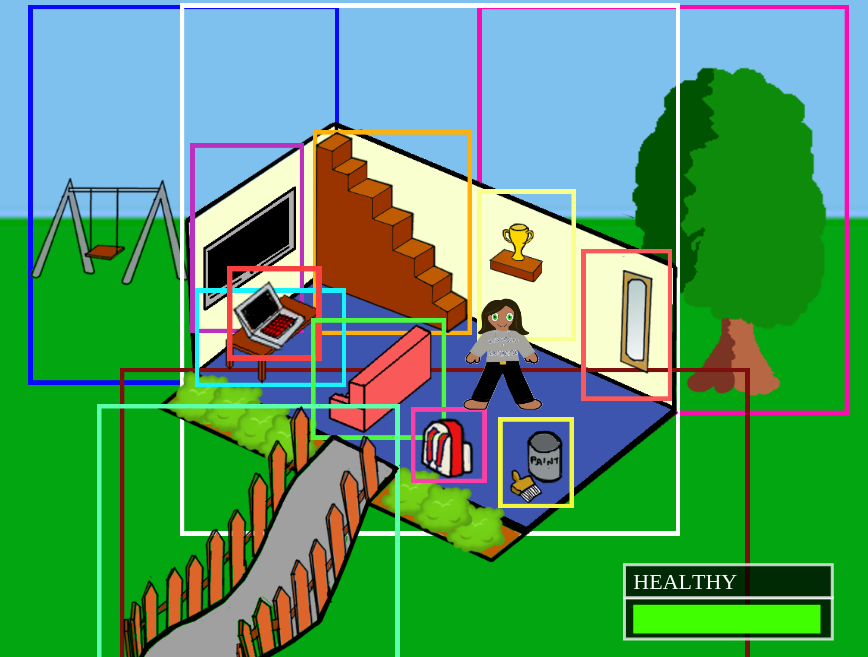
\includegraphics[width=0.80\linewidth]{Artist_Guide_Images/hub_outlines}
	\caption{Hub Item Positions}
	\label{fig:hub_outlines}
\end{figure}

\subsection{Avatar Items}
\label{subsec:avatar_items}
Avatars are created by directly layering the five components on top of each other. As such, please do not use all of the space, but rather position the item so it will align with the other components, and leave the remainder of the space with the transparent background.

\begin{table}[H]
	\centering
	\begin{tabular}{|c|c|}
		\hline
		Item &		Dimensions \\ \hline
		Eyes &		1000 x 1000 \\
		Head &		1000 x 1000 \\
		Skin &		1000 x 1000 \\
		Shirt &		1000 x 1000 \\
		Trousers &	1000 x 1000 \\ \hline
	\end{tabular}
	\caption{Avatar Sprite Dimensions}
	\label{tab:avatar_dimensions}
\end{table}

\subsection{Carriable Items}
\label{subsec:carriable_items}

The images will be completely square when displayed, so ensure any designed images are square and please use transparency to fill in any excess space.

\end{document}
